\chapter{Introduction}
	This bachelor project has been produced by Tomas Alan Lieberkind and Asger Schlichtkrull from the 1st February 2013 to the 22nd May 2013 at the IT-University of Copenhagen. The project has been supervised by Peter Sestoft.

\section{Motivation}
	We would like to improve development of web applications with ASP.NET Web Forms and therefore it is beneficial to investigate how JavaScript can be safely represented in order to acheive compile time validation.

	Developing web applications instead of native applications is a strong tendency in software development today. JavaScript contributes to enriching the user experience and sometimes provide functionality which is indispensable for such web applications.

	ASP.NET Web Forms provides the possibility of building HTML documents with C\# which improves correctness through compile time validation. Writing JavaScript code from C\# is not possible in the same way as with HTML. JavaScript is embedded into the application as hard coded text strings and thus compile time validation is not possible. This increases the possibility of writing faulty code that emits errors which are not discovered before client side runtime. Runtime errors are generally harder to debug and in worst case exposed to the end user while leaving the application in a corrupt state.

	Achieving compile time validation of JavaScript is not a ground-breaking thought, and there are several existing projects that do exactly this; TypeScript by Microsoft and Dart by Google are just a few.

	Depending on the problem at hand one weakness with those solutions could be that the server side code and the client side code (JavaScript) is written as two independent units, and nothing ties them safely together. Essentially server side code and client side code is compiled separately. 

	Another problem is that of reusability. In cases such as form validation it is necessary to write the same piece of code in two different languages in order to validate both on client side and server side.

	This project aims to find a solution that incorporates compile time validation, generation of client side code from server side code, and safely tying client and server side together.

\section{Reading Guide}

	This report is directed to people with interest in how JavaScript can be safely written in ASP.NET WebForms projects. It is assumed that the reader has a general understanding of Abstract Syntax Trees for representing programs source code and a basic understanding of JavaScript. Third party libraries used in the project, namely Roslyn and Script\#, will be introduced and thus knowledge about these is not a prerequisite.

	TODO: NÆVN MICS

	This document consists of six chapters.

	Chapter one introduces the project, the motivation behind it and its scope. Additionally it introduces the case study upon which it is based.

	Chapter two briefly introduces ASP.NET Web Forms and the usage of Code Behind to develop web applications. Furthermore it explains why JavaScript can be considered an unsafe language.

	Chapter three introduces various technologies that can be useful to the project and describes how they can be used in combination to approach the project in different ways. Furthermore an analysis is conducted in order to investigate which approach is most convenient to implement.

	The MiCS project is an implementation of the approach chosen in chapter three. Chapter four describes the MiCS project in details, starting with the overall flow needed to convert C\# to JavaScript, the architecture of the project, the implementation of the stages described in the flow and correctness testing of the project.

	Chapter five and six evaluates the solution from chapter four, reflects on the design goals set in the problem definition and discusses what direction the project should take from here.

\section{Problem definition}
	The problem definition has changed since the beginning of this project. Originally we wanted to represent JavaScript as an internal DSL in C\#. Instead we widened our perspective, to include other possible approaches to safe JavaScript development in ASP.NET Web Forms. Below, the revised problem definition is listed.
	\begin{itemize}

	\item Study JavaScript and describe its unsafe language features.

	\item Investigate how JavaScript can be safely represented within ASP.NET Web Forms. This includes compile time validation and how to activate the generated JavaScript in a safe manner (client-server side consistency).

	\item Investigate how to implement a solution that generates JavaScript from server side code (client-server side portability).

	\item Implement and test a class library that supports safe JavaScript development from Code Behind.


	\end{itemize}



	\subsection{Learning goals}
		\begin{itemize}

		\item Better knowledge of JavaScript in general and the more subtle language features of the language.
		\item Better knowledge of ASP.NET Web Forms.
	 	\item Better understanding of the difference between C\#/.NET (as a static typed) language and JavaScript (dynamically typed language).
		\item Better understanding of web development and the communication between client and server side...
		\item Basic knowledge of cross compilers and abstract syntax trees.
		\end{itemize}

\section{Method}
	\begin{itemize}
	\item We will study JavaScript literature to obtain a better understanding JavaScript and which of its features can be considered unsafe. 
	\item We will investigate what technologies and libraries can contribute to the project and how these combined can be used to approach solutions in different ways.
	\item We will analyse and compare the solutions in order to find the one that best fits this project
	\item We will design and implement the solution from step 2.
	\item We will set up a unit test suite in order to ensure that everything works as expected.
	\end{itemize}

\section{Scope}
	As a complete mapping from C\# to JavaScript is unrealistic to implement in the given period of time, the project is based on a case study. Only the subset of C\# needed to fulfill the requirements set by the case study will be taken into account.

	\subsection{Case Study}
		A very common use case of JavaScript is form validation. As a user experience enriching feature, forms are often validated on client side, as to avoid the waiting time for a page load (e.g.\ JavaScript can be disabled in the browser). However, forms have to be validated on the server side as well as the client side validation is easily bypassed. Our case study concerns the validation of a registration form. Specifically, we would like to be able to:

		\begin{itemize}
			\item Validate strings using Regular Expressions to check if email addresses, postal addresses and phone numbers are correctly formatted
			\item Validate the length of strings to check that users do not enter an exceptionally long string, e.g. for their name
			\item Validate something based on the choice of something else
		\end{itemize}

		Figure~\ref{registrationForm} shows the registration form, and below, the validation criteria are explained.

		\begin{figure}
			\begin{center}
				\centerline{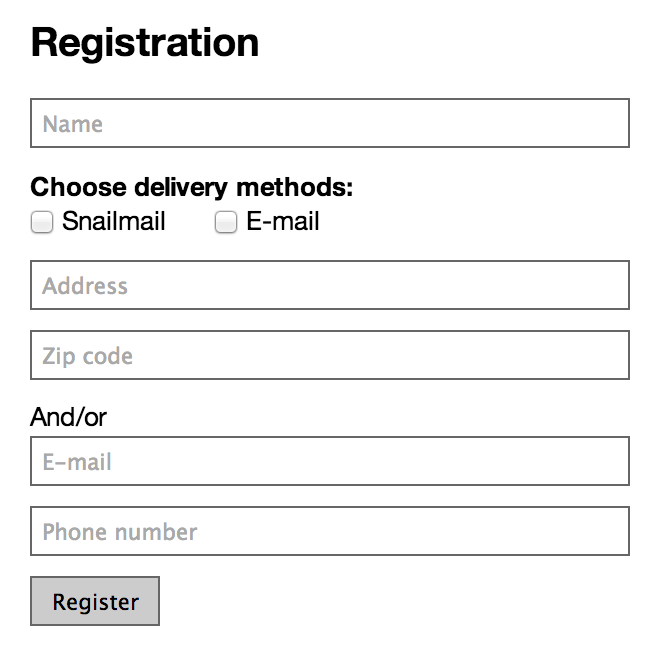
\includegraphics[width=7cm]{resources/images/registrationform.png}}
			\end{center}
			\caption{The form that we aim at validating}
			\label{registrationForm}
		\end{figure}

		\begin{itemize}
			\item The name has to consist of at least a first name and a last name, cannot be less than 5 characters long and not exceed 128 characters
			\item At least one delivery method has to be checked. If “Snailmail” is checked, the address and zip code fields have to be filled in. If “E-mail” is checked, the “E-mail” field has to be filled in.
			\item The address has to follow the format: \newline\newline \texttt{(streetname) (house number)[, (floor number). (TH|TV|SAL)]}\newline\newline where everything within the brackets is optional. For example, the addresses ``Amagerbrogade 125, 3.TV'' and ``Englodden 4'' are valid addresses whereas ``Griffenfeldsgade'' and ``Svinget 34, 4'' are not.
			\item The zip code has to consist of four characters (Danish zip code).
			\item The e-mail has to be a valid e-mail
			\item The phone number has to consist of 8 numbers, where the first number cannot be “0”.
		\end{itemize}

	\subsection{Focus}
		The project primarily serves as a proof-of-concept and therefore the main focus will be to generate code that actually works, and can fulfill the requirements set by the case study. Performance and the quality of the generated code will not be assessed. 

		TODO: Nævn at fokus er på ASP.NET platformen og ikke andre.

\section{Target Audience}
	The target audience are developers who write web applications using ASP.NET Web Forms and C\# where correctness is of high priority. This implies that the developer wants to display a 100\% working application to his end users or nothing at all (or maybe an error message). It is better to show an error message than to display an application which can exist in a corrupt, or partly corrupt, state.


